%!TEX root = ../thesis.tex
% ******************************* Thesis Appendix B ********************************
\graphicspath{{Appendix1/}}
\chapter{Frequency-dependent MC Method}
\section*{Introduction}
Actually, a typical MC simulation strategy for phonon transport is relatively the same as what we used in our MC simulation:we initialize, launch, and trace phonon
ensembles in terms of temperature, frequency, polarization, and
positions. Local temperature distribution varies depending on the
positions of these ensembles.Typically, because there we will take abut the simulation considering dispersion and polarization, which results in the different treatment in phonon scattering mainly.
The simulation starts by initializing all the
phonon ensembles (including those to be launched from the constant-
temperature boundary and within the material due to heat
generation at each $\Delta$t). These ensembles are moved ballistically
from one position to another within the time interval of $\Delta$t, assuming
that ensemble properties remain unaltered. Ensembles that hit
a constant-temperature boundary are recorded in terms of energy
for heat flux calculation and then deleted. Those that encounter an
insulated surface are assumed to be reflected specularly or diffusively.
Otherwise, ensembles reside at the corresponding locations
after the ballistic movement.Once the propagation phase is complete,
local temperature distribution is calculated based on the
positions of the ensembles. It is important to notice that local phonon
distribution function after the propagation phase is different
from the equilibrium distribution (i.e., the Bose–Einstein distribution).Only the local distribution of total phonon energy is known.
Although a medium can still be in a non-equilibrium state, it is
possible to calculate ‘pseudo-temperature’ distribution\cite{BTE1} assuming
that equilibrium exists.\\
 Next, we will give a introduction to frequency-dependent MC based on Wong's work\cite{wongMC}.
\section*{Method}
\subsection*{Phonon descriptions - dispersion relation, density of states, and group velocity}
The data points of the dispersion relation for silicon are provided
by Brockhouse\cite{brockhouse}.And Wong gives quadratic expressions to fit the dispersion data.Thus,calculating
the angular frequency with known wave vector or vice versa can
be achieved easily during a MC simulation. 
\begin{figure}[htbp!] 
\centering    
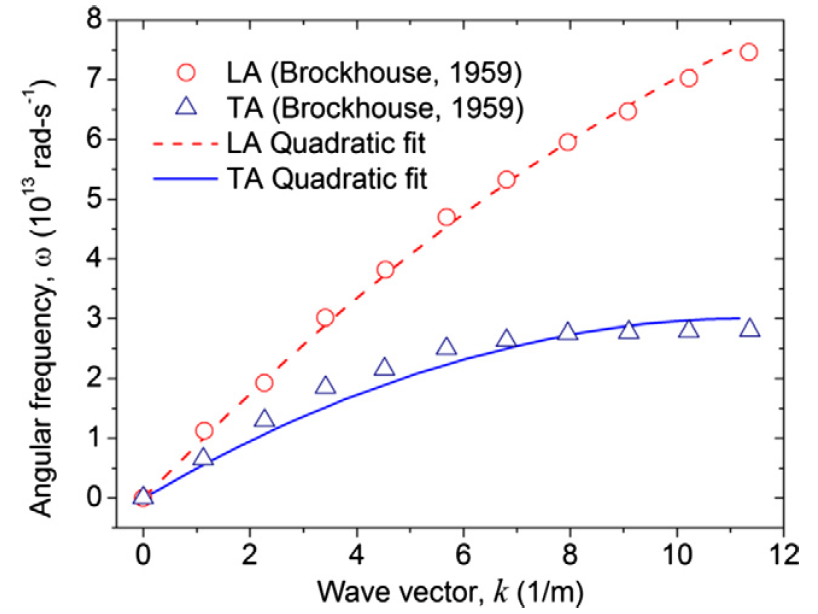
\includegraphics[width=0.6\textwidth]{dispersion}
\caption[Phonon Dispersion of Silicon]{Data points of the dispersion relation of silicon obtained from Brockhouse\cite{brockhouse}.}
\label{fig:dispersion}
\end{figure}
\indent And the quadratic expressions
for the LA- and TA-dispersion relations are obtained as:
\begin{equation}
\omega=9280k - 2.234 \times 10^{-7} k^2 (LA) \label{con:1}
\end{equation}
\begin{equation}
\omega= 5240k - 2.278 \times  10^{-7} k^2 (TA) \label{con:2}
\end{equation}
When the dispersion relation is known, the phonon density of states for a given polarization branch, $D(\omega,p)$, is calculated as:
\begin{equation}
D(\omega ,p)=\frac{k^2}{2 \pi v_g(\omega,p)}
\end{equation}
And the group velocity of the phonon, $v_g(\omega,p)$ can be calculated as:
\begin{equation}
v_g(\omega,p)=\frac{\partial \omega}{\partial k}   \label{con:4}
\end{equation}
\subsection*{Determining properties of phonon ensembles – quantity,
frequency, velocity, and polarization}
To start a MC simulation, the required number of statistical
ensembles needs to be specified and initialized. This is done by
first calculating the total actual number of phonons present in
the medium. Since a ‘‘reference temperature’’ is set in the simulation,
only phonons that are created beyond the reference are initialized.
Therefore, the initial number of phonons available for
carrying excess heat in the medium above the reference is calculated
as:
\begin{equation}
N_{ph,ini}=XYZ \sum_p \sum_i [f_0(\omega_i,T_{ini},p)-f_0(\omega_i,T_{ref},p)]D(p,\omega_i)\Delta \omega_i
\end{equation}
where the index p includes two transverse acoustic (TA) and one
longitudinal acoustic (LA) polarization branches of phonons.
And a scaling
factor, Wscaling, is used to represent the actual number of phonons
that each statistical ensemble carries:
\begin{equation}
W_{scaling}=\frac{N_{ph,ini}}{N_{en,m}}
\end{equation}
where $N_{en,m}$ is the initial number of statistical ensembles used to represent the total actual number of phonons present in the medium. At each time step, $\Delta$, the excess number of phonons emitted from a boundary with constant temperature of $T_R$ or $T_L$ in reference to $T_{ref}$ at each time step is computed as:
\begin{equation}
N_{ph,R}=XY {\Delta t} \sum_p \sum_{i=1}^{N_b}[f_0( \omega_i,T_R)-f_0( \omega_i,T_{ref})][ \vec{v_g}( \omega_i) \times \hat{n}]D( \omega_i,p) \Delta \omega_i
\end{equation}
where $(\vec{v_{\omega,g}} \times \hat{n})$ is the phonon group velocity normal to the boundary. Thus, the scaling factor becomes:
\begin{equation}
W_{scaling}=\frac{N_{ph,R}}{N_{en,R}}
\end{equation}
The next step is to determine the frequency of a phonon ensemble
launched from the $T_R$-boundary. This is done by first constructing
the CPDF of the number of phonons over the frequency spectrum
as:
\begin{equation}
R_i=\sum_{j=1}^i N_j / \sum_{j=1}^{N_b} N_j  \label{con:R}
\end{equation}
where
\begin{equation}
N_j=\Delta \omega _j  \lbrace [f_0(\omega_j,T_R) - f_0(\omega_j,T_{ref})] D(\omega_j, LA) +2 D(\omega_j, TA) \rbrace 
\end{equation}
In Eq(\ref{con:R}), the frequency spectrum is divided into $N_b$ intervals. Then a random number, denoted as $Ran_{\omega}$, si drawn such that:
\begin{equation}
R_{i-1} < Ran_{\omega} < R_i
\end{equation}
and the actual frequency of the statistical ensemble is calculated as:
\begin{equation}
\omega = \omega_i + (2 Ran_{\omega} - 1) \frac{\Delta \omega_i}{2}
\end{equation}
At last, when the frequency of the ensemble is known, we can then determine its polarization bu computing the ratio of the LA-phonons to the total number of phonons n all polarization branches in the $\omega$ interval, which is given as:
\begin{equation}
P_{LA,i}=\frac{[f_0(\omega_i,T_R)-f_0(\omega_i,T-{ref})]D(\omega_i,LA)}{[f_0(\omega_i,T_R)-f_0(\omega_i,T_{ref})][D(\omega_i,LA)+2D(\omega_i,TA)]}
\end{equation}
A random number, $Ran_P$, is then drawn to compare with $P_{LA}$,i. If $Ran_P$
is less than $P_{LA}$,i, then the ensemble belongs to the LA polarization
branch; otherwise, it belongs to the TA polarization branch. The
same procedures are applicable for the $T_L$-boundary. With the frequency
and polarization branch known, the group velocity of the
ensemble can be determined easily using Eqs. (\ref{con:1}), (\ref{con:2}), and (\ref{con:4}).

\subsection*{Sampling initial launching and scattering angles,tracking algorithms}
The same with the MC method we used.
\subsection*{'Pseudo-temperature' calculation}
Once the statistical ensembles of phonons start to propagate
and interchange between small control volumes (or computational
elements) within the entire computation domain, the resultant local
phonon distribution loses its thermodynamic equilibrium. In
order to calculate the local temperature, however, it is necessary
to assume that the total energy carried by ensembles of phonons
in a local computational element is equal to the total phonon energy
computed using the Bose–Einstein distribution for the same
volume. The temperature obtained under such condition is called
as a ‘pseudo-temperature’, denoted as $T_{pseudo}$.Therefore, the following
equation needs to be solved for the $T_{pseudo}$ at each time step:
\begin{equation}
\sum_p \sum_{i=0}^{N_b} \hbar \omega_i [f_0(\omega_i,T_{pseudo})-f_0(\omega_i,T_{ref}]D_i(\omega_i,p) \Delta \omega_i = \frac{E(x,y,z)}{\Delta x \Delta y \Delta z }
\end{equation}
which varies locally.$E(x,y,z)$ is the local energy carried by phonon ensembles within a computational element with $(\Delta x \Delta y \Delta z)$ volume.
\subsection*{Phonon scattering treatment in MC simulation}
Here we go to the most important part. Scattering of phonons consists of two types, following either a
Normal (N) or an Umklapp (U) process\cite{Ashcroft,Ziman,zimanphonons}.
Both processes
tend to restore equilibrium; however, only U-processes resist heat
conduction. In this work, only three-phonon scattering is accounted
during MC simulation although it is probable that fourphonon
scattering and beyond may occur at high temperatures,
which will be left to future studies. In the three-phonon scattering
processes, two phonons can be combined to yield one phonon or a
phonon can be decomposed into two separate phonons. Both Nand
U-processes follow energy conservation as:
\begin{equation}
\hbar \omega_1 + \hbar \omega_2 \leftrightarrow \hbar \omega_3 \label{con:30}
\end{equation}
The indices 1, 2, and 3 indicate three different phonons, respectively,
and the process given in Eq(\ref{con:30}) is reversible.
In addition,
phonon scattering follows momentum conservation. For N-process,
it is given as:
\begin{equation}
k_1 + k_2 \leftrightarrow k_3
\end{equation}
The $k$'s are the wave vectors of phonons. For U-process, it follows that:
\begin{equation}
k_1 + k_2 \leftrightarrow k_3 + G
\end{equation}
where $G$ is the lattice reciprocal vector. Details and physics involved
in phonon scattering will not be further discussed here because
they are covered extensively in any solid state physics books.
\indent In the current MC simulation, the parameter involved to account
for the phonon scattering is the total relaxation time (i.e.,
$\tau-{NU}$), which includes both N- and U-processes. According to the
Mathiessen rule, it is given as\cite{Ashcroft,zimanphonons}:
\begin{equation}
\frac{1}{\tau_{NU}}=\frac{1}{\tau_{N}}+\frac{1}{\tau_{U}}
\end{equation}
Thus, the CPDF of phonon scattering between $t$ and $t + \Delta t$ is written as:
\begin{equation}
R_{scat} = 1- exp (\frac{- \Delta t}{\tau_{NU}})
\end{equation}
In order to determine if a phonon ensemble is scattered after a time
step of $\Delta t$, a random number $Ran_{scat}$ is drawn and compared to $R_{scat}$. If $R_{scat}$ is less than $R_{scat}$, the ensemble is scattered. Hence Hence ensemble
frequency, polarization, and direction are reset. Relaxation times
are typically temperature and frequency dependent; therefore,
these quantities are to be calculated at each time step. For silicon,
these properties are well-documented. Here, we can use the relaxation
times expressions proposed by Holland\cite{hollandanalysis} for three-phonon scattering
and employed by many researchers in MC simulations\cite{monte1,monte2} since these expressions produced good fit for the thermal
conductivity of silicon in different temperature range. The inverse
relaxation times for N- and U-processes are given as follows:
\begin{equation}
LA-phonons \quad  and\quad N or U-process \rightarrow \tau_{LA,NU}^{-1}=B_l \omega^2 T^3
\end{equation}


\begin{equation}
TA-phonons \quad  and\quad N-process \rightarrow \tau_{TA,N}^{-1} =
\begin{cases}
B_T \omega^2 T^4 & \forall \omega < \omega_{1/2}\\
0 & \forall \omega \geq \omega_{1/2}
\end{cases}
\end{equation}

\begin{equation}
TA-phonons\quad  and\quad  U-process \rightarrow \tau_{TA,U}^{-1} =
\begin{cases}
0 & \forall \omega < \omega_{1/2}\\
\frac{B_{TU} \omega^2}{sinh(\hbar \omega / k_B T)} & \forall \omega \geq \omega_{1/2}
\end{cases}
\end{equation}
where $B_L, B_T, and B_{TU}$ are constants to be determined using bulk
thermal conductivity data, and x1/2 is the frequency corresponding
to $k/k_{max}$ = 0.5 based on the $TA-dispersion$ curve. The values of these
constants will be given in the chart\cite{chen2005monte}.\\

\begin{table}[!hbp]
\centering
\begin{tabular}{|c|c|}
\hline $B_T$  &$9.3 \times 10^{-13}$ \\
\hline $B_L$ &  $1.0 \times 10^{-30} (deg^{-3}s)$ \\
\hline $B_{TU}$&$5.50 \times 10^{-18} s$\\
\hline    
\end{tabular}\\
\caption{B parameters}
\end{table}

\noindent During the process of phonon scattering, the frequency/energy
of each scattered phonon ensemble is reset while additional energy
may be added or removed. Thus it is crucial to include an additional
step to counteract this imbalance of energy within a control
volume. A destruction/creation scheme for phonons can be implemented
to prevent any excess energy gain or loss, and the added/
deleted phonons are to be drawn from the equilibrium phonon distribution\cite{BTE1}.

\subsection*{Accounting external heat generation}
Heat generation is included in our MC simulation by implementing
a phonon creation scheme. It is assumed that the type
of heat generation, whether Joule, laser or electron-beam heating,
is not important as long as the rate of phonon production by the
source is known. This requires the distribution of the volumetric
power generated within the material,$g^{'''}(x,y,z)$,to be determined
before the MC simulation. When
$g^{'''}(x,y,z)$ is known, the amount
of energy generated within each computational element and at
each time step is calculated as:
\begin{equation}
E_{gen}(x,y,z)=g^{'''} \Delta x \Delta y \Delta z \Delta t
\end{equation}
Then just add $E_{gen}$ to the item $E$.

%%%%%%%%%%%%%%%%%%%%%%%%%%